\begin{theorem}
    \hypertarget{thrm4.18}{(Предел композиции 2)} Пусть $f: U_{\sigma_{0}} (y_{0}) \mapsto \R, \  y: \mathring{U}_{\delta_{0}} (x_{0}) \mapsto U_{\sigma_{0}}(y_{0}). $

    Пусть $f$ непрерывна в точке $y_0$ и $\lim\limits_{x \to x_{0}} y(x) = y_{0}$, Тогда:
    $$ \exists \lim\limits_{x \to x_{0}} f \circ y(x) = \lim\limits_{x\to x_{0}} f(y(x)) = f(y_{0})
    $$
\end{theorem} 
\begin{proof}
    $$\begin{cases}
        \forall \epsilon > 0 \ \exists \sigma(\epsilon) \in (0, \sigma_{0}): \ \forall y \in U_{\sigma(\epsilon)}(y_{0}) \hookrightarrow |f(y) - f(y_{0})| < \epsilon \\
        \forall \sigma > 0 \ \exists \delta(\sigma) \in (0, \delta_{0}): \ \forall y \in U_{\delta(\sigma)}(x_{0}) \hookrightarrow |y(x) - y_{0}| < \sigma            
    \end{cases}$$

    Объединяя высказывания, получим:

    $$
    \forall \epsilon > 0 \ \exists \widetilde{\delta}(\epsilon)=\delta(\sigma(\epsilon)) \in (0, \delta_{0})
    $$
    $$
    \forall x \in \mathring{U}_{\widetilde{\delta}_{\epsilon}}(x_{0}) \hookrightarrow y(x) \in U_{\sigma(\epsilon)}(y_{0}),\quad \textrm{а значит} \quad |f(y(x)) - f(y_{0})| < \epsilon
    $$

    В итоге, получаем:
    $$ \forall \epsilon > 0 \ \exists \widetilde{\delta}(\epsilon) \in (0, \delta_{0}): \forall x \in \mathring{U}_{\delta(\epsilon)}(x_{0}) \hookrightarrow  |f(y(x)) - f(y_{0})| < \epsilon \Leftrightarrow \exists\lim\limits_{x \to x_{0}} f(y(x)) = f(y_{0}).
    $$
\end{proof}

\begin{corollary}
    Если $f: U_{\sigma_{0}} (y_{0}) \mapsto \R,$ где $y_{0} = y(x_{0}),  \ \ y: U_{\delta_{0}}(x_{0}) \mapsto \R,$ то $\exists \ \overline{\delta} \in (0, \delta_{0}): f \circ y$ определена в некоторой $U_{\overline{\delta}}(x_{0})$ и $f \circ y$ непрерывна в точке $x_0$.
\end{corollary}
\begin{proof}
    Так как $y$ непрерывна в $y_{0} = y(x_{0}) \Rightarrow \exists \lim\limits_{x \to x_{0}} y(x) = y_{0}$.

    Значит, $\exists \overline{\delta} > 0: \ \forall x \in U_{\overline{\delta}}(x_{0}) \hookrightarrow y(x) \in U_{\sigma_{0}}(y_{0}) \Rightarrow f \circ y(x) \  \textrm{определена} \ \forall x\in U_{\overline{\delta}}(x_{0})$

    Так как $f$ непрерывна в точке $y_{0}$ и $y(x) \to y_{0} = y(x_{0}), x \to x_{0}$, можно воспользоваться предыдущей теоремой. Получается, 
    $$ \lim\limits_{x\to x_{0}} f(y(x)) = f(y_{0}) = f(y(x_{0}))
    $$
    Следовательно, $f \circ y$ непрерывна в точке $x_{0}$
\end{proof}

\subsection{Обратная функция}

\begin{lemma}
    $f: X \mapsto Y$~---~обратима на $X$, когда $f$~---~сюръекция и инъекция.
\end{lemma}
\begin{proof}
    
    \underline{Шаг 1.} Пусть $f$~---~сюръекция и инъекция, докажем, что $f$ обратима. 
    
    Рассмотрим $y \in Y$. Так как $f$~---~сюръекция, $\exists x\in X: f(x) = y.$ Но так как $f$~---~инъекция, то этот $x$ единственный ($\forall x' \neq x \ f(x') \neq f(x) = y$). Следовательно, определим $f^{-1}(y) = x$ (единственный). В одну строну доказали.

    \underline{Шаг 2.} Пусть $f$ обратима, докажем, что $f$~---~сюръекция и инъекция.

    Так как $f$ обратима, то $\exists f^{-1}: Y \mapsto X \Rightarrow f$~---~сюръекция.
    $$\forall y \in Y \ \exists x = f^{-1}(y): f(f^{-1}(y)) = f(x) = y.$$

    Покажем, что $f$~---~инъекция. Возьмем $x_{1}, x_{2} \in X$
    $$ f(x_{1}) = f(x_{2}) = y \Rightarrow f^{-1}(f(x_{1})) = f^{-1}(f(x_{2})) = f^{-1}(y) \Rightarrow x_{1} = x_{2}.
    $$
\end{proof}

\begin{lemma}
    \hypertarget{lemm4.9}{Пусть $X \subset \R, X \neq \varnothing$. Пусть $f$: $X \mapsto \R$ строго монотонна. Тогда $f$ обратима, то есть $\exists f^{-1}: f(X) \mapsto X.$}

    Более того, если $f$ строго возрастает на $X$, то $f^{-1}$ строго возрастает на $f(X)$. Если $f$ строго убывает на $X$, то $f^{-1}$ строго убывает на $f(X)$.
\end{lemma}

\begin{note}
    Лемма неверна, если не требовать строгой монотонности.
\end{note}
\begin{example}
    $ f(x) \equiv 1 $ на $\R$. Это нестрого монотонная функция и она необратима на $\R$.
\end{example}
\begin{proof}
    Из строгой монотонности $f$ следует, что $f$: $X \mapsto f (X)$ инъективно (так как иначе $\exists x_{1}, x_{2} \in X$: $x_{1} < x_{2}$ и $f (x_{1}) = f (x_{2})$, то есть нарушается строгая монотонность).

    Рассмотрим случай возрастания на $X$, так как случай строго убывания аналогичен.

    Обратная $f^{-1}$: $f(X) \mapsto X$ существует в силу инъективности $f$ (сюръективность очевидна, так как мы используем отображение в $f (X)$). Покажем, что она тоже строго возрастает. Возьмём $y_{1}, y_{2} \in f(X)$. Пусть $y_{2} > y_{1}$. Предположим, что $f^{-1} (y_{2}) < f^{-1}(y_{1})$ (равно быть не может в силу обратимости $f$)

    Так как $f$ строго возрастает, то $f\Bigl(f^{-1}(y_{2})\Bigr) < f\Bigl(f^{-1}(y_{1})\Bigr)$, то есть $y_{2} < y_{1}$. Получили противоречие c нашим предположением, следовательно, $\forall y_{1}, y_{2} \in f(X)$ из $y_{1} < y_{2} \Rightarrow f^{-1}(y_{1}) < f^{-1}(y_{2}).$ То есть обратная функция имеет тот же характер монотонности.
\end{proof}

\begin{theorem}
    \hypertarget{thrm4.19}{(Об обратной функции)}
    Пусть $f \in \text{C} \big([a, b]\big)$ строго монотонна на $[a, b]$. Тогда $\exists f^{-1} \in \text{C} \big( [m, M]\big)$ (где $m = \underset{x \in [a, b]}{min} f (x)$, а $M = \underset{x \in [a, b]}{max} f (x)$) и имеет характер монотонности тот же, что и у $f$.
\end{theorem}
\begin{proof}
    Тот факт, что $\exists f^{-1}$ и она имеет тот же характер монотонности, что $f$, вытекает из \hyperlink{lemm4.9}{предыдущей леммы}.
    
    $f([a, b]) = [m, M]$ следует из \hyperlink{thm5.4}{теоремы Больцано-Коши}.

    Остаётся показать $f^{-1} \in \text{С} \left([m, M]\right)$. Рассмотрим случай $y_{0} \in \Bigl(m, M \Bigr)$

    Так как $y_{0} \in \Bigl(m, M \Bigr)$, то $x_{0} \in (a, b)$. Зафиксируем $\epsilon > 0$ такое, что $U_{\epsilon}(x_{0}) \subset (a, b).$

    Рассмотрим отрезок $[x_{0} - \epsilon, x_{0} + \epsilon] \subset (a, b)$. На нём $f$ строго возрастает и непрерывна.

\begin{center}
\scalebox{0.65}{
        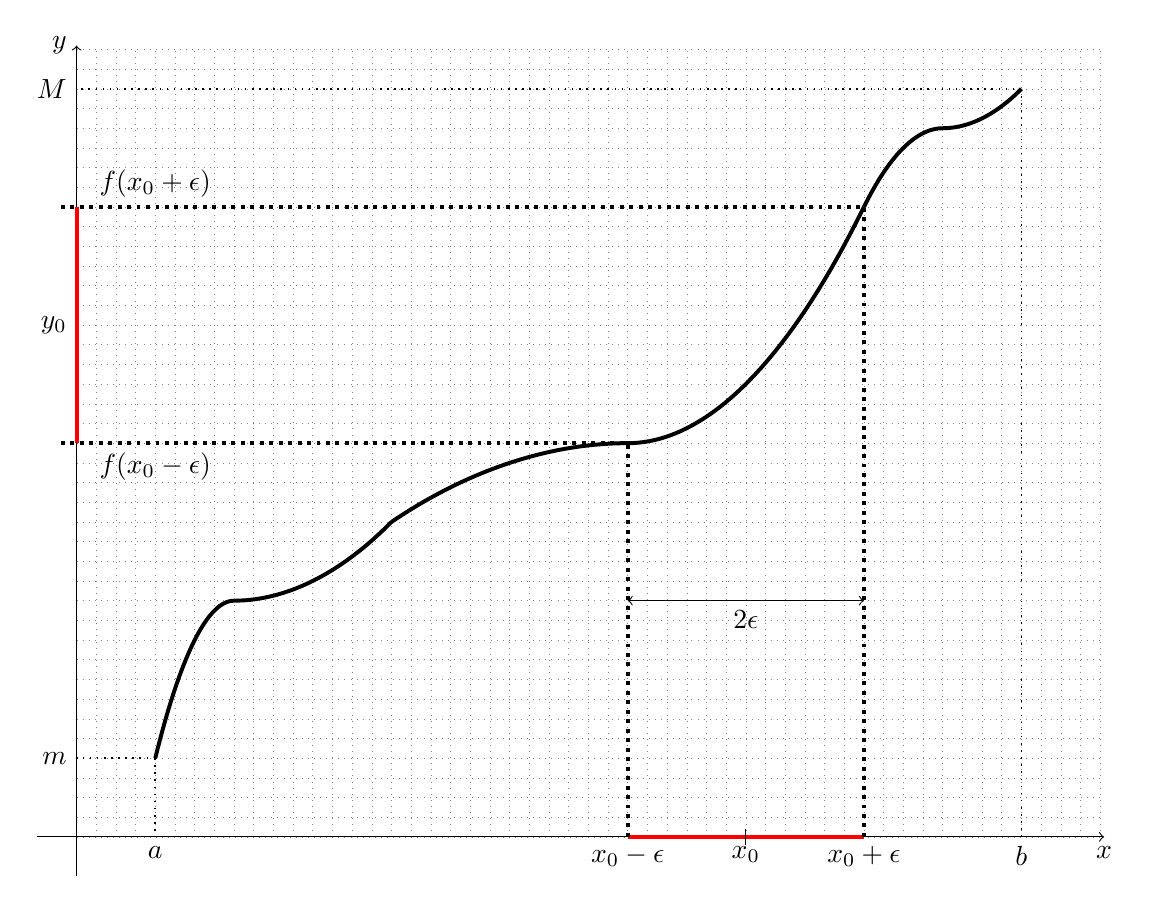
\begin{tikzpicture}
    % Рисуем сетку
    \draw[help lines, step=0.25, dotted]
    (-6,-5) grid (7,5);
    % Начало координат
    \draw[->, thin] (-6.5,-5) -- (7.05,-5)
    node[below] {$x$}; % Ox
    \draw[->, thin] (-6, -5.5) -- (-6, 5.05)
    node[left] {$y$}; % Oy

    \draw[line width =.05cm](-5, -4) parabola bend (-4, -2) (-2, -1);
    \draw[line width =.05cm](-2, -1) parabola bend (1, 0) (4, 3);
    \draw[line width =.05cm](4, 3) parabola bend (5, 4) (6, 4.5);

    \draw[line width =.05cm, red] (-6, 0) -- (-6,3);
    \draw[line width =.05cm, red] (1, -5) -- (4, -5);

    \draw[dotted, line width =.02cm] (-5, -4) -- (-5, -5);
    \draw[dotted, line width =.02cm] (-5, -4) -- (-6, -4);
    \draw[dotted, line width =.02cm] (6, 4.5) -- (6, -5);
    \draw[dotted, line width =.02cm] (6, 4.5) -- (-6, 4.5);
    \draw[dotted, line width =.05cm] (-6.2, 0) -- (1, 0);
    \draw[dotted, line width =.05cm] (1, -5) -- (1, 0);
    \draw[dotted, line width =.05cm] (-6.2, 3) -- (4, 3);
    \draw[dotted, line width =.05cm] (4, -5) -- (4, 3);

    \draw[] (2.5, -5.1) -- (2.5, -4.9);
    \draw[<->] (1, -2) -- (4, -2);

    \node[below] at (2.5, -2){$2\epsilon$};
    \node[below] at (1, -5) {$x_{0} - \epsilon$};
    \node[below] at (4, -5) {$x_{0} + \epsilon$};    
    \node[below] at (2.5, -5){$x_{0}$};
    \node[left] at (-6, -4) {$m$};
    \node[left] at (-6, 4.5) {$M$};
    \node[left] at (-6, 1.5) {$y_{0}$};
    \node[below] at (-5, -5) {$a$};
    \node[below] at (6, -5) {$b$};
    \node[right, below] at (-5, 0) {$f(x_{0} - \epsilon)$};
    \node[right, above] at (-5, 3) {$f(x_{0} + \epsilon)$};
    \end{tikzpicture}
}
\end{center}
    
    Следовательно, $f$ осуществляет биекцию $[x_{0} - \epsilon, x_{0} + \epsilon]$ на  $[f(x_{0} - \epsilon), f(x_{0} + \epsilon)]$
    $$ \delta(\epsilon) = \min \{ f(x_{0}) - f(x_{0} - \epsilon), f(x_{0} + \epsilon) - f(x_{0})\}.
    $$

    Рассмотрим интервал $\Bigl( f(x_{0}) - \delta(\epsilon), f(x_{0}) + \delta(\epsilon) \Bigr) \subset \Bigl( f(x_{0} - \epsilon), f(x_{0} + \epsilon) \Bigr) \Rightarrow$
    $$\Rightarrow
    \forall y \in \Bigl( f(x_{0}) - \delta(\epsilon), f(x_{0}) + \delta(\epsilon) \Bigr) \hookrightarrow f^{-1}(y) \in U_{\epsilon}(x_{0}) = U_{\epsilon}\Bigl(f^{-1}(y_{0})\Bigr)
    $$
    
    Следовательно, $f^{-1}$ непрерывна в точке $y_{0}$.

    Для концевых точек аналогично, только в них будет односторонняя непрерывность.
\end{proof}

\begin{corollary}
    Пусть $f \in C\Bigl([a, b] \Bigr), a, b \in \Hat{\R}$ и строго монотонна. Тогда $\exists f^{-1} \in C\Bigl( (m, M )\Bigr)$ и строго монотонна с тем же характером монотонности, что и у $f$.
%    $$m = \underset{x\in (a, b)}{\inf} f(x) \in \Hat{\R}
 %   $$
 %   $$M = \underset{x\in (a, b)}{\sup} f(x) \in \Hat{\R}
 %   $$
\end{corollary}
\begin{proof}
    Так как $f$ строго монотонна, то $\exists f^{-1},$ имеющая тот же характер монотонности. Покажем, что $f\Bigl((a,b)\Bigr) = \Bigl(m, M \Bigr).$

    $$m = \underset{x\in (a, b)}{\inf} f(x) \in \Hat{\R}
    $$
    $$M = \underset{x\in (a, b)}{\sup} f(x) \in \Hat{\R}
    $$
    
    В силу \hyperlink{thrm4.15}{обобщённой теоремы о промежуточном значении}. 
    $$f\Bigl((a,b)\Bigr) \supset \Bigl(m, M \Bigr).$$

    Но $m$ и $M$ не могут приниматься. Рассмотрим случай строгого возрастания (для убывания аналогично). 
    
    $$\textrm{Если}\ \exists x^{*} \in (a, b): \  M = f(x^{*}) \Rightarrow \exists x^{**} \in (x^{*}, b): f(x^{**}) > f(x^{*}) = M,$$ 
    
    но это противоречит тому, что $M = \underset{x\in (a, b)}{\sup} f(x). \Rightarrow f\Bigl((a, b\Bigr)) \subset \Bigl(m, M \Bigr) \Rightarrow $
    $$\Rightarrow f\Bigl((a, b)\Bigr) = \Bigl(m, M \Bigr).$$

    Непрерывность $f^{-1}$ доказывается так же, как в предыдущей теореме.
\end{proof}


\subsection{Первый замечательный предел и непрерывность элементарных функций}
\begin{note}
    В этом параграфе утверждения доказываются неточно (но для экзамена и так сойдёт).
\end{note}

\sidefig(10 cm)(7 cm)
{
 \normalsize{\begin{lemma}
     $$\sin x < x < \tg x, \quad x \in \Bigl(0, \cfrac{\pi}{2} \Bigr)$$
 \end{lemma}}
 \begin{proof}
     $$S_{OAB} < S_{\textrm{сектора}} < S_{OAC}$$
     $$\cfrac{\sin x}{2} < \cfrac{x}{2} < \cfrac{\tg x}{2}$$
 \end{proof}
 }
{
    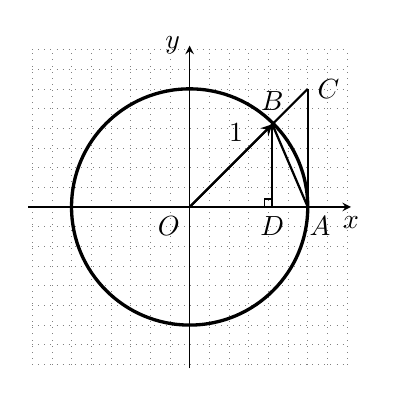
\begin{tikzpicture}[>=stealth]
    % Рисуем сетку
    \draw[help lines, step=0.25, dotted]
    (-2,-2) grid (2,2);
    % Рисуем окружность
    \draw[very thick] (0,0) circle (1.5);
    % Начало координат
    \draw[->, thin] (-2.05,0) -- (2.05,0)
    node[below] {$x$}; % Ox
    \draw[->, thin] (0,-2.05) -- (0,2.05)
    node[left] {$y$}; % Oy

    \draw[thick] (0,0)  -- (1.5, 1.5);
    \draw[->, thick] (0,0)  -- (1.05, 1.05);
    \draw[thick] (1.05,0)  -- (1.05, 1.05);
    \draw[thick] (1.5,0)  -- (1.05, 1.05);
    \draw[thick] (1.5,0)  -- (1.5, 1.5);

    \draw[line width =.015cm] (0.95,0)  -- (0.95, 0.1) -- (1.05, 0.1);
    \node[below left] at (0,0) {$O$};
    \node[below] at (1.05,0) {$D$};
    \node[below right] at (1.4,0) {$A$};
    \node[left] at (0.8,0.95) {$1$};
    \node[above] at (1.05, 1.1) {$B$};
    \node[right] at (1.5,1.5) {$C$};
    \end{tikzpicture}
}
\begin{corollary}
    \hypertarget{cor4.2}{(Первый замечательный предел)} 

    $$\exists \lim\limits_{x \to 0} \frac{\sin x}{x} = 1$$
\end{corollary}
\begin{proof}
    Так как мы работаем в проколотой окрестности  нуля, то $\cfrac{\sin x}{x}$ определена. В силу принципа локализации достаточно считать, что мы изучаем $\cfrac{\sin x}{x}$ в интервале $\Bigl( -\cfrac{\pi}{2}, \ \cfrac{\pi}{2}\Bigr)\  \backslash\  \{0\}$;  $\cfrac{\sin x}{x}$~---~чётная.    

    $$
    \cfrac{\sin x}{\tg x} < \cfrac{\sin x}{x} < 1 \Leftrightarrow \ \cos x  < \cfrac{\sin x}{x} < 1 \quad \forall x \in \Bigl(0, \cfrac{\pi}{2}\Bigr)
    $$

    В силу чётности:

    $$\cos x  < \cfrac{\sin x}{x} < 1 \quad \forall x \in \Bigl(-\cfrac{\pi}{2}, \cfrac{\pi}{2}\Bigr) \quad (*)
    $$

    В силу непрерывности $\cos x$ в нуле $\exists \lim\limits_{x \to 0} \cos x = \cos 0 = 1$.
    
    Пользуясь $(*)$ и \hyperlink{thm4.7}{теоремой о двух милиционерах}  получаем, что $\exists \lim\limits_{x \to 0} \frac{\sin x}{x} = 1$
\end{proof}

\begin{theorem}
    $\sin x$ и $\cos x$ непрерывны по всей своей области определения.
\end{theorem}
\begin{proof}
    В силу \hyperlink{thrm4.18}{теоремы о композиции непрерывных функций} достаточно доказать непрерывность синуса в каждой точке, так как $\cos x = \sin \Bigl(x + \cfrac{\pi}{2} \Bigr)$.
    
    $\forall x_{1}, x_{2} \in \R$: $|\sin x_{1} - \sin x_{2}| = \left|2 \sin \left( \cfrac{x_{1} - x_{2}}{2} \right) \cos \left( \cfrac{x_{1} + x_{2}}{2} \right)\right| \leq 2 \left| \sin \left( \cfrac{x_{1} - x_{2}}{2} \right) \right| \leq 2 \cdot \cfrac{|x_{1} - x_{2}|}{2} = |x_{1} - x_{2}|$

    Следовательно, если зафиксировать $x_{0}$, то
    $$ 0 \leq |\sin x - \sin x_{0}| \leq |x - x_{0}| \to 0, x\to x_{0}.$$

    По \hyperlink{thm4.7}{теореме о двух милиционерах} $\lim\limits_{x \to x_{0}} \sin x = \sin x_{0}. $
\end{proof}

\begin{definition}
    Функция $\arcsin x$ по определению обратна к $\sin x$ на отрезке $\left[-\cfrac{\pi}{2}, \cfrac{\pi}{2}\right]$

    Она существует, так как $\sin x$ монотонен и непрерывен на отрезке $\left[-\cfrac{\pi}{2}, \cfrac{\pi}{2}\right]$ 

    Следовательно, $arcsin x$ строго возрастает и непрерывна на $[-1, 1].$
\end{definition}
\begin{definition}
    Функция $\arccos x$ по определению обратна к $\sin x$ на отрезке $\left[0, \pi\right]$

    Она существует, так как $\cos x$ монотонен и непрерывен на отрезке $\left[0, \pi\right]$.

    Следовательно, $arccos x$ строго убывает и непрерывна на $[-1, 1].$
\end{definition}

     \begin{tikzpicture}[>=stealth]
    \begin{axis}[
    domain=-1:1, 
    samples=500, 
    axis lines*=middle, 
    xtick={-1,1}, 
    ytick={-1.57,1.57}, 
    yticklabels={$-\pi$/2,$\pi$/2},
    grid = minor]
    \addplot[color = red]  {asin(x)/180*pi};
    \addplot[dotted]  {x};
    \addplot[color = blue]  {sin(x*180/pi)};
      \end{axis}
    \end{tikzpicture}
    \begin{tikzpicture}[>=stealth]
    \begin{axis}[
    domain=-1:1, 
    samples=500, 
    axis lines*=middle, 
    ytick={-1,1.57, 3.14}, 
    yticklabels={-1,$\pi$/2,$\pi$},
    grid = minor]
    \addplot[color = red]  {acos(x)/180*pi};
      \end{axis}
    \end{tikzpicture}